%!TEX root = ../main.tex

\section{Modeling approach}

Engineering correlations, reduced-order models, and CFD modeling techniques were used to investigate the effects of recycled gas on the operation of a fluidized-bed biomass pyrolysis reactor. The following sections discuss approaches implemented in this work for calculating gas properties and the associated effects on fluidization conditions and pyrolysis yields.

\subsection{Gas properties}

Density of the gas is calculated from the ideal gas law as shown in Equation \ref{eq:density} where $\rho_{gas}$ is density (kg/m$^3$), $P$ is pressure (Pa), $MW$ is molecular weight (g/mol), $R$ is the gas constant [(m$^3$ Pa) / (K mol)], and $T$ is temperature (K).

\begin{equation}\label{eq:density}
    \rho_{gas} = \frac{P\,MW}{R\,T}
\end{equation}

Gas viscosity ($\mu_{gas}$ as \textmugreek P) is determined from Equation \ref{eq:viscosity}, thermal conductivity ($k_{gas}$ as W/m\,K) is estimated from Equation \ref{eq:thermlcond}, and heat capacity (C$_{p\,gas}$ as J/mol\,K) is calculated from Equation \ref{eq:heatcap}. Temperature of the gas in Kelvin is represented by $T$ while the regression coefficients $A$, $B$, $C$, $D$, $E$, $F$, and $G$ for each gas are obtained from Yaws' Handbook \cite{Yaws2014}.

\begin{equation}\label{eq:viscosity}
    \mu_{gas} = A + B\,T + C\,T^2 + D\,T^3
\end{equation}

\begin{equation}\label{eq:thermlcond}
    k_{gas} = A + B\,T + C\,T^2 + D\,T^3
\end{equation}

\begin{equation}\label{eq:heatcap}
    C_{p\,gas} = A + B\,T + C\,T^2 + D\,T^3 + E\,T^4 + F\,T^5 + G\,T^6
\end{equation}

Several methods are available to calculate the viscosity of a gas mixture. Equation \ref{eq:graham} calculates the mixture viscosity from the sum of the mole fraction and viscosity product of each gas component in the mixture \cite{Graham-1846} while Equation \ref{eq:herning} accounts for the molecular weight of each gas component \cite{Herning-1936}.

\begin{equation}\label{eq:graham}
    \mu_{mix} = \sum(x_i \cdot \mu_i)
\end{equation}

\begin{equation}\label{eq:herning}
    \mu_{mix} = \frac{\sum(\mu_i \cdot x_i \cdot \sqrt{MW_i})}{\sum(x_i \cdot \sqrt{MW_i})}
\end{equation}

\subsection{Fluidization correlations}

For a bed of particles, the minimum fluidization velocity $U_{mf}$ is the gas velocity at which the drag force of the upward moving gas equals the weight of the particles. Kunii and Levenspiel \cite{Levenspiel-1991} provide the following equation for calculating minimum fluidization velocity

\begin{equation}
    U_{mf} = \frac{Re_{p,mf} \mu}{d_p \rho_g}
\end{equation}

\noindent where $\mu$ is gas viscosity (kg/m\,s), $d_p$ is particle diameter (m), $\rho_g$ is gas density (kg/m$^3$), and $Re_{p,mf}$ is the particle Reynolds number (-) at minimum fluidization conditions. The Reynolds number is calculated from the Archimedes number ($Ar$) and two dimensionless constants ($a, b$) which represent experimental coefficients. Different $U_{mf}$ correlations were evalutaed based on experimental data from Wen and Yu where $(a, b) = (33.7, 0.0408)$, from Richardson where $(a, b) = (25.7, 0.0365)$, and from Grace where $(a, b) = (27.2, 0.0408)$ \cite{Levenspiel-1991}.

\begin{align}
    Re_{p,mf} &= \left( a^2 + b Ar \right)^{1/2} - a \\
    Ar &= \frac{d_p^3 \rho_g (\rho_s - \rho_g) g}{\mu^2}
\end{align}

According to Kunii and Levenspiel \cite{Levenspiel-1991}, the constants ($a, b$) can be derived from the Ergun pressure drop equation based on the constants $K_1$ and $K_2$ where $\epsilon_{mf}$ is the bed void fraction (-) at minimum fluidization and $\phi$ is sphericity (-) of the bed particles. For this paper, $U_{mf}$ is estimated based on the Ergun, Grace, Richardson, and Wen and Yu correlations.

\begin{equation}
    a = \frac{K_2}{2 K_1} \qquad
    b = \frac{1}{K_1}
\end{equation}

\begin{equation}
    K_1 = \frac{1.75}{\epsilon_{mf}^3 \phi} \qquad
    K_2 = \frac{150(1-\epsilon_{mf})}{\epsilon_{mf}^3 \phi^2}
\end{equation}

\subsection{Pyrolysis kinetics}

A pyrolysis kinetics scheme based on the work of Di Blasi was implemented to predict the conversion of biomass into gas, tar, and char products \cite{Blasi-1993,Blasi-2001}. Figure \ref{fig:blasi} gives an overview of the scheme and its reaction mechanisms. Reactions 1--3 represent the primary conversion of biomass while reactions 4--5 are secondary reactions that reduce tar yield at long residence times.

\begin{figure}[H]
    \centering
    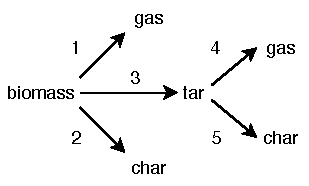
\includegraphics[width=0.4\textwidth]{blasi.pdf}
    \caption{Diagram of the Di Blasi pyrolysis kinetics scheme for conversion of biomass to gas, tar, and char products.}
    \label{fig:blasi}
\end{figure}

The pyrolysis reactions were modeled as first-order Arrhenius type equations where the reaction rate is given as

\begin{equation}
    r_i = C_i\,A_i\,e^{-E_i / R\,T}
\end{equation}

\noindent where $r_i$ is the rate of reaction $i$ such that $C_i$ is a mass based concentration, $A_i$ is the pre-factor (1/s), $E_i$ is the activation energy (kJ/mol), $R$ is the gas constant, and $T$ is the reaction temperature (K). Kinetic parameters for each reaction are listed in Table \ref{tab:kinetic-params} where $\Delta H$ is the heat of reaction (kJ/kg).

\begin{table}[H]
    \centering
    \caption{Kinetic parameters for the Di Blasi biomass pyrolysis scheme.}
    \begin{tabular}{clrrc}
        \toprule
        Reaction    & A (1/s)               & E (kJ/mol) & $\Delta$H (kJ/kg) & Reference \\
        \midrule
        1           & $4.38 \times 10^9$    & 152.7      & -20               & \cite{Blasi-2001} \\
        2           & $3.27 \times 10^6$    & 111.7      & -20               & \cite{Blasi-2001} \\
        3           & $1.08 \times 10^{10}$ & 148.0      & 255               & \cite{Blasi-2001} \\
        4           & $4.28 \times 10^6$    & 108.0      & -42               & \cite{Blasi-1993} \\
        5           & $1.00 \times 10^6$    & 108.0      & -42               & \cite{Blasi-1993} \\
        \bottomrule
    \end{tabular}
    \label{tab:kinetic-params}
\end{table}

\subsection{CFD-DEM simulation}

A coarse-grained CFD-DEM model was implemented for biomass pyrolysis in MFiX, an open-source, Fortran-based code [X]. The implemented coarse-grained CFD-DEM model in this research is an extension of the standard MFiX release. Gas phase transport was described using conservation equations of mass, momentum, energy, and chemical species in the Eulerian framework (Equations \ref{eq:gas-trans-mass}--\ref{eq:gas-trans-chemical}, respectively).

\begin{align}
    \frac{d(\epsilon_g \rho_g)}{dt} + \nabla (\epsilon_g \rho_g u_g) &= S_\rho \label{eq:gas-trans-mass} \\
    \frac{d(\epsilon_g \rho_g u_g)}{dt} + \nabla (\epsilon_g \rho_g u_g u_g) &= -\epsilon_g \nabla p + \nabla (\epsilon_g \tau) + \epsilon_g \rho_g g + S_u \\
    \frac{d(\epsilon_g \rho_g E)}{dt} + \nabla (\epsilon_g \rho_g u_g E) &= -\nabla Q + S_E \\
    \frac{d(\epsilon_g \rho_g Y_i)}{dt} + \nabla (\epsilon_g \rho_g u_g Y_i) &= -\nabla (D_i \nabla Y_i) + S_{Y_i} \label{eq:gas-trans-chemical}
\end{align}

where $\epsilon_g$, $\rho_g$, $u_g$, $p$, $\tau$, $Q$, and $Y_i$ are gas phase volume fraction, density, velocity, pressure, stress tensor, conductive heat flux, and ith chemical species, respectively, $t$ is time, $g$ is acceleration due to gravity, $D_i$ is mass diffusion coefficient for species, $S_\rho$, $S_u$, $S_E$, and $S_{Y_i}$ are mass, momentum, energy, and chemical species source terms, respectively. Fixed quantities of discrete particles with identical initial conditions were lumped into a computational coarse-grained parcel (CGP), whose motion was governed by Newton’s second law of motion. All particle forces and contact dynamics were calculated on the parcel scale, whereas heat and mass transfers were calculated on particle scale and projected to the entire parcel. Accordingly, all particles in same coarse- grained parcel possess identical temperature, chemical species concentration, and momentum. The mass and diameter of each coarse-grained parcel was such that:

\begin{align}
    m_{CGP} &= m_p W \\
    d_{CGP} &= d_p W^{1/3}
\end{align}

where $m_{CGP}$ is CGP mass, $m_p$ is distinct particle mass, $W$ parcel statistical weight, $d_{CGP}$ is CGP diameter, and $d_p$ is distinct particle diameter. Instantaneous accelerations (translational and rotational) for each coarse-grained parcel were calculated as:

\begin{align}
    \frac{d u_{CGP}}{dt} &= g - \frac{F_p}{m_{CGP}} + \frac{F_c}{m_{CGP}} + \frac{F_d}{m_{CGP}} \\
    \frac{d \omega_{CGP}}{dt} &= \frac{T_{CGP}}{I_{CGP}}
\end{align}

where $u_{CGP}$ and $\omega_{CGP}$ are the CGP translational and rotational velocities, $g$ is acceleration due to gravity, $m_{CGP}$ is CGP mass, $T_{CGP}$ is net torque on the CGP, and $I_{CGP}$ is CGP moment of inertia. The term $F_p$ represents pressure gradient force and is calculated as product of the CGP volume and pressure gradient. The CGP collision forces $F_C$ (parcel-parcel and parcel-wall collisions) was modeled according linear spring-dashpot model \cite{Navarro-2013}. Since the number of CGP collisions is significantly lower than the number of collisions expected in system with distinct particles, the CGP coefficient of restitution was modified as a correction for energy dissipations during collisions. The proposed modification to the CGP coefficient of restitution is calculated following kinetic theory of granular flow \cite{Lu-2014} as:

\begin{equation}
    e_{CGP} = \sqrt{1 + (e_p^2 - 1) W^{1/3}}
\end{equation}

where $e_{CGP}$ is CGP coefficient of restitution and $e_p$ is distinct particle coefficient of restitution. Two different drag models were used to estimate CGP drag force $F_d$ based on well-documented difference in the fluidization behavior of sand and biomass in the literature \cite{Oliveira-2013}. Drag force was estimated following Ganser-corrected Gidaspow drag model for sand (bed material) particles and a filtered drag model for biomass particles. Th Ganser correction \cite{Ganser-1993} was coupled to the Gidaspow model \cite{Gidaspow-1994} to account for non-sphericity of the sand particles as expressed below:

\begin{equation}
    \beta_{Ganser} =
    \begin{cases}
        \beta_{Ergun} & \text{if } \epsilon_g \leq 0.8 \\
        \beta_{WenYu} & \text{if } \epsilon_g > 0.8
    \end{cases}
\end{equation}

\begin{align}
    \beta_{Ergun} &= 150 \frac{(1 - \epsilon_g)^2 \mu_g}{\epsilon_g d^2_{CGP} \phi^2} + 1.75 \frac{(1 - \epsilon_g) \rho_g}{\epsilon_g d_{CGP} \phi} |u_g - u_{CGP}| \\
    \beta_{WenYu} &= \frac{3}{4} C_d \frac{(1 - \epsilon_g) \rho_g}{d_{CGP} \phi} |u_g - u_{CGP}| \epsilon_g^{-2.65}
\end{align}

\begin{equation}
    C_d =
    \begin{cases}
        \frac{24}{Re K_1} (1 + 0.1118(Re K_1 K_2)^{0.6567}) + \frac{0.4305 K_2}{1 + \frac{3305}{Re K_1 K_2}} & \text{if } Re < 1,000 \\
        0.44 & \text{if } Re \geq 1,000 \\
        0.0 & \text{if } Re = 0.0
    \end{cases}
\end{equation}

\begin{align}
    K_1 &= \left(\frac{1}{3} + \frac{2}{3} \phi^{-0.5} \right)^{-1} - 2.25 \frac{d_{CGP}}{D} \\
    K_2 &= 10^{1.8148 (-log \phi)^{0.5743}}
\end{align}

The filtered drag model (modified Sarkar drag model) used in this research for biomass particles was proposed by Gao et al. \cite{Gao-2018} and was found by the authors to have relatively high prediction strength across multiple flow regimes in fluidized bed. The modified Sarkar drag model is derived fine-grid simulation with Wen-Yu drag model and can be computed as:

\begin{equation}
    \beta_{Sarkar} = \beta_{WenYu} (1 - H_{Sakar})
\end{equation}

\begin{equation}
    H_{Sakar} =
    \begin{cases}
        0.95 \left(1 - e^{-\alpha_1 \alpha_2 (u_{\text{slip}}^* - u_0)^p} \right) & u_{\text{slip}}^* > u_0 \\
        0.0 & u_{\text{slip}}^* \leq u_0
    \end{cases}
\end{equation}

\begin{equation}
    u_{\text{slip}}^* = \frac{|u_g - u_{CGP}|}{u_t}
\end{equation}

\begin{align}
    \alpha_1 &= \frac{\left(a_1 + a_2(1 - \epsilon_g) + a_3(1 - \epsilon_g)^2 + a_4(1 - \epsilon_g)^3 + a_5(1 - \epsilon_g)^4 \right)}{1 + e^{100 \left((1 - \epsilon_g) - 0.55 \right)}} \\
    \alpha_2 &= \left(1 + \frac{a_6}{\Delta_{\text{filter}}^*} + \frac{a_7}{(\Delta_{\text{filter}}^*)^2} \right) \left(1 + \frac{a_8}{(u_{\text{slip}}^*)^2} \right)
\end{align}

\begin{equation}
    u_0 = \frac{a_9 + a_{10} (1 - \epsilon_g)}{0.01 + (1 - \epsilon_g)^{a_{11}}} \left(1 + \frac{a_{12}}{\Delta_{\text{filter}}^*} + \frac{a_{13}}{(\Delta_{\text{filter}}^*)^2} \right)
\end{equation}

\begin{equation}
    p = \left(a_{14} + a_{15}(1 - \epsilon_g) + a_{16}(1 - \epsilon_g)^2 \right) \left(1 + \frac{a_{17}}{\Delta_{\text{filter}}^*} + \frac{a_{18}}{(\Delta_{\text{filter}}^*)^2} \right)
\end{equation}

\begin{align}
    \Delta_{\text{filter}}^* &= max\left( \frac{g \Delta_{\text{filter}}}{u_t^2}, \; \frac{1}{2} \right) \\
    \Delta_{\text{filter}} &= 2 (\Delta_x \times \Delta_y \times \Delta_z)^{1/3}
\end{align}

\begin{equation}
    u_t = \frac{g d_{CGP}^2 (\rho_{CGP} - \rho_g)}{18 \mu_g}
\end{equation}

\begin{equation}
    \begin{matrix}
        a_1    & a_2    & a_3 \\
        a_4    & a_5    & a_6 \\
        a_7    & a_8    & a_9 \\
        a_{10} & a_{11} & a_{12} \\
        a_{13} & a_{14} & a_{15} \\
        a_{16} & a_{17} & a_{18} \\
    \end{matrix}
    \; =
    \begin{array}{rrr}
        0.75597773   & 2.73931487  & -5.60196497 \\
        -1.65853820  & 16.70299223 & -0.44145335 \\
        0.18195034   & -0.01827347 & 0.28441799  \\
        -1.943573770 & 0.22177961  & 0.31175890  \\
        -0.15971960  & 0.47750002  & 0.062794180 \\
        5.13011673   & 0.67680355  & -0.54535726 \\
    \end{array}
\end{equation}
